\documentclass[../main.tex]{subfiles}

\begin{document}
\graphicspath{{../imagenes/opamp/}}
\renewcommand{\subsectionbreak}{}
\section{Amplificadores Operacionales}
	\subsection{Introducción}
	Un Op-Amp es un dispositivo electrónico del tipo activo que tiene la capacidad de
	amplificar la señal en sus bornes de entrada (alta ganancia) entre otras cosas.
	Dependiendo de la configuración elegida en sus pines se lo puede usar como un
	comparador de señales (entre sus 2 entradas), amplificador inversor y no inversor,
	seguidor de tensión, sumador y hasta derivado – integrador de señales, entre las más
	comunes y útiles.


	\subsection{Particularidades constructivas}
	La estructura interna de un amplificador consta básicamente en 3 etapas, amplificaciones
	en cascada (agrupadas en la etapa de entrada, amp. diferencial), amplificación de tensión
	y la salida.

	\begin{itemize}
		\item Impedancia de entrada: resistencia entre las entradas del rango de los M$\Omega$.
		\item Impedancia de salida: resistencia vista desde la salida del rango de los $\Omega$.
		\item Ganancia en lazo abierto: ganancia de tensión del rango de los 100000 a 500000
		veces.
		\item Ancho de banda (bandwidth): rango de frecuencias que el dispositivo acepta (que
		puede amplificar).
		\item Tensión de offset: diferencia de potencial entre las entradas del Op-Amp para
		llevar la tensión de salida al valor nulo. Del rango de los mv.
		\item Corriente de polarización: necesaria para polarizar las entradas, del rango de los
		nA.
		\item Diferencia de potencial de alimentación: en general, ronda los 30 V entre pines
		de alimentación (puede ser fuente partida o fuente simple con un pin a masa).
	\end{itemize}


	\begin{figure}[H]
		\centering
		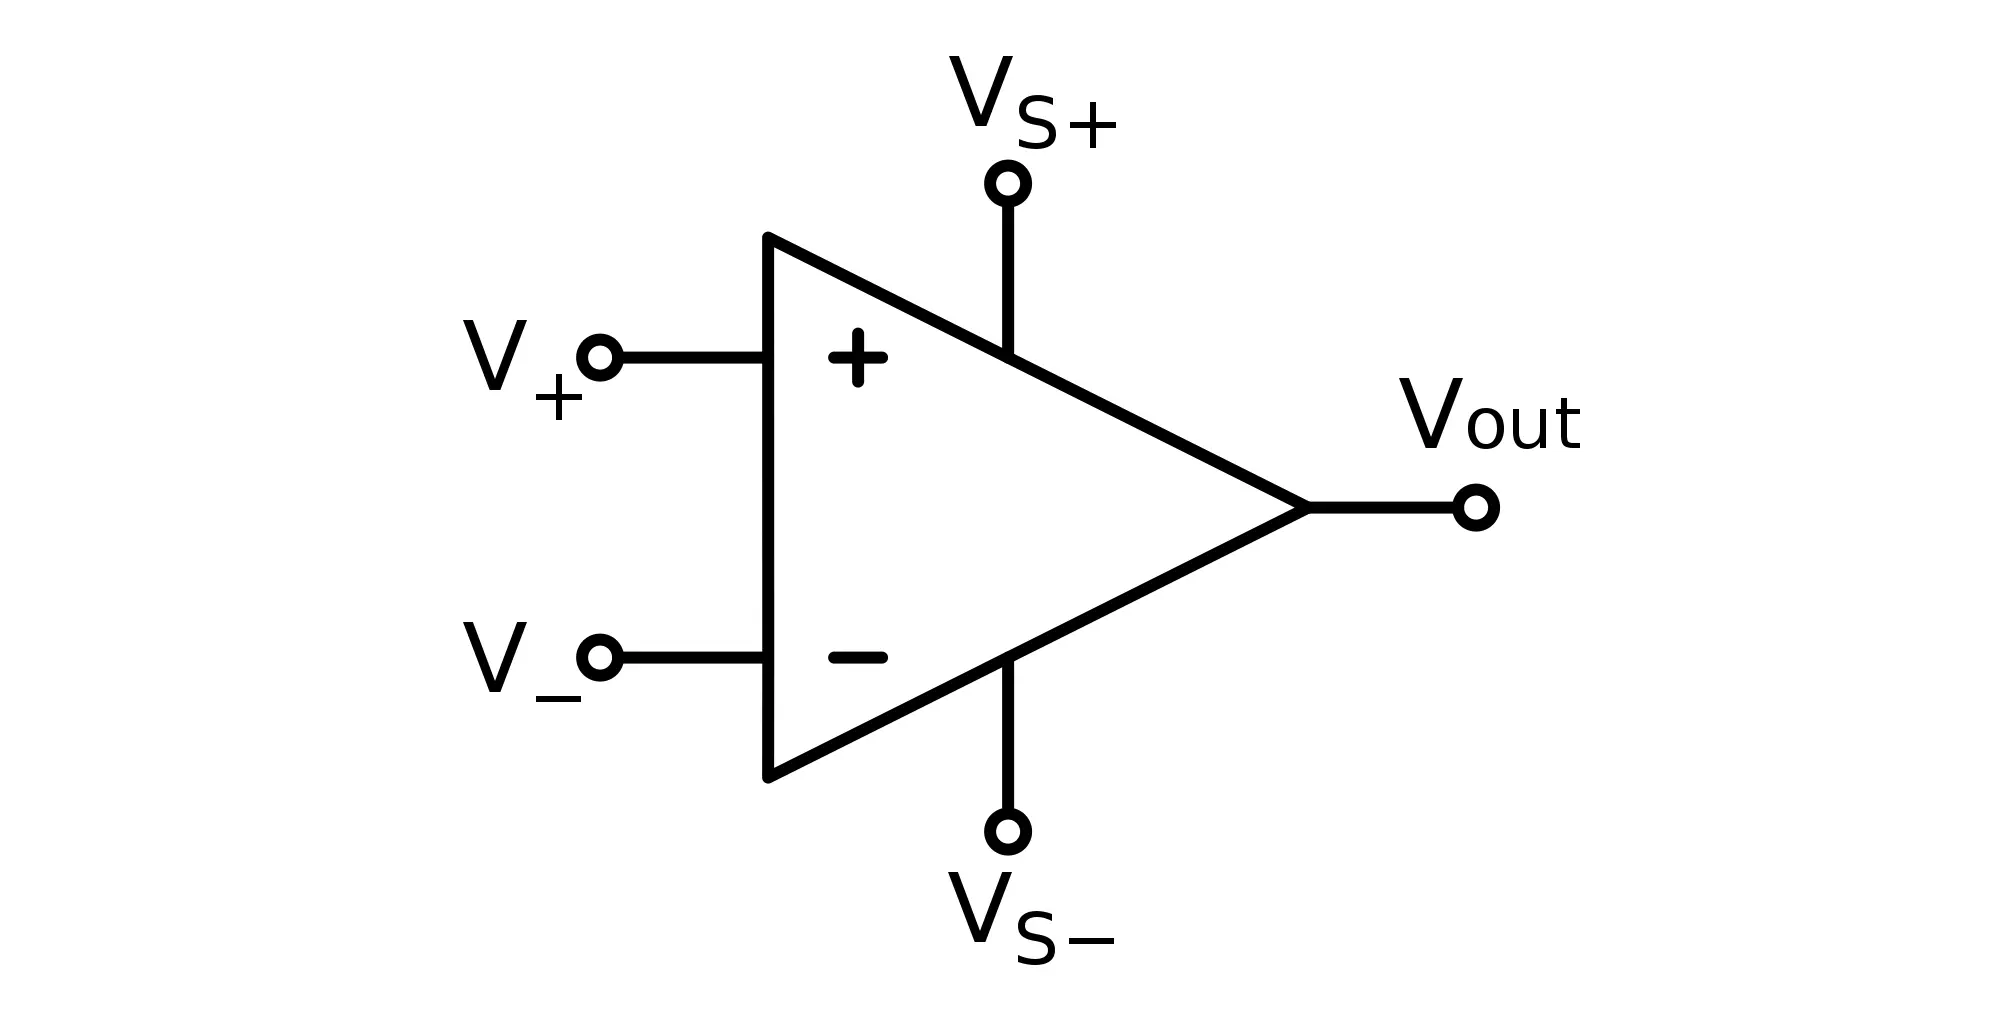
\includegraphics[width=0.5\textwidth]{imagen1.png}
		\caption{Simbolo eléctrico del amplificador operacional}
	\end{figure}

	Donde
	\begin{itemize}
		\item $V_+$: entrada no inversora
		\item $V_-$: entrada inversora
		\item $V_{out}$: salida del Op-Amp
		\item $V_{S+}$: fuente de alimentacion positiva
		\item $V_{S-}$: fuente de alimentacion negativa (o masa)
	\end{itemize}

\clearpage
	\subsection{Configuraciones}
	Circuitos y Ecuaciones particulares:
%--------------------------------------------------------------
		\subsubsection{Comparador}
		\begin{figure}[H]
			\centering
			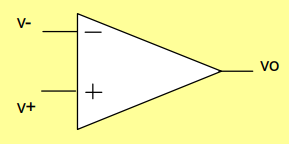
\includegraphics[width=0.45\textwidth]{imagen2.png}
			\caption{Un amplificador operacional en configuración comparador}
		\end{figure}
		Si la tensión en la entrada no inversora ($V+$) es mayor a la tensión de la inversora
		($-V_+$), la salida será la tensión de alimentación positiva ($+VCC$). En caso
		contrario la salida será $-VCC$ .
		\[
			V_+ > V_- \longrightarrow V_{out} = +V_{CC}
		\]
		\[
			V_- > V_+ \longrightarrow V_{out} = -V_{CC}
		\]
%--------------------------------------------------------------
		\subsubsection{Amplificador Inversor}
		\begin{figure}[H]
			\centering
			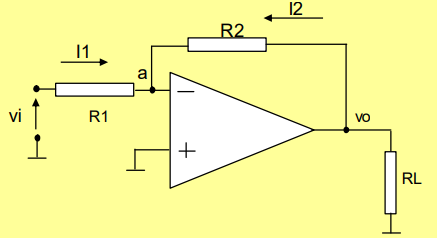
\includegraphics[width=0.45\textwidth]{imagen3.png}
			\caption{Un amplificador operacional en configuración inversor}
		\end{figure}
		La ganancia nos viene dada por los valores de las resistencias, según la expresión
		siguiente:
		\[
			\text{Ganancia de Tensión} = \dfrac{V_{out}}{V_{in}} = - \dfrac{R_2}{R_1}
		\]
		El signo negativo se debe que la salida esta desfasada 180° con respecto a la señal
		de entrada.

%--------------------------------------------------------------
		\subsubsection{Amplificador no Inversor}
		\begin{figure}[H]
			\centering
			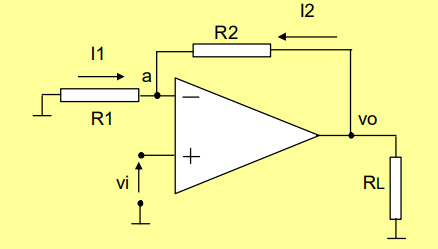
\includegraphics[width=0.45\textwidth]{imagen4.png}
			\caption{Un amplificador operacional en configuración no inversor}
		\end{figure}
		La ganancia nos viene dada por los valores de las resistencias, según la expresión
		siguiente:
		\[
		\text{Ganancia de Tensión} = \dfrac{V_{out}}{V_{in}} = 1 + \dfrac{R_2}{R_1}
		\]

%--------------------------------------------------------------
		\subsubsection{Seguidor de tensión}
		\begin{figure}[H]
			\centering
			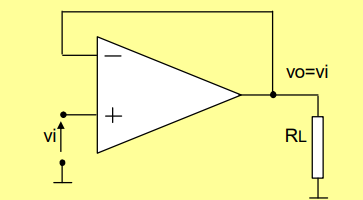
\includegraphics[width=0.45\textwidth]{imagen5.png}
			\caption{Un amplificador operacional en configuración seguidor de tensión}
		\end{figure}
		Esta configuración permite ofrecer alta impedancia de entrada al generador de
		señal V In y no modifica su valor en la salida.
		\[
		\text{Ganancia de Tensión} = \dfrac{V_{out}}{V_{in}} = 1
		\]
%--------------------------------------------------------------
		\subsubsection{Sumador}
		\begin{figure}[H]
			\centering
			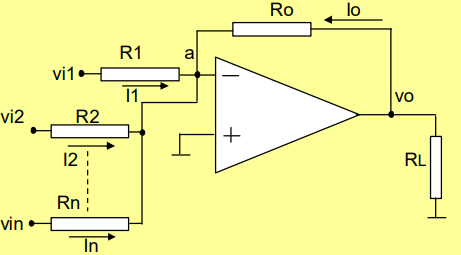
\includegraphics[width=0.45\textwidth]{imagen6.png}
			\caption{Un amplificador operacional en configuración sumador} 
		\end{figure}
		\[
			V_{out} = R_0 \x 
			\left(
				\dfrac{V_1}{V_{R1}} + \dfrac{V_2}{V_{R2}} + \dfrac{V_n}{V_{Rn}} 
			\right)
		\]

	\clearpage
	\subsection{Componente Activo}
	Debido a que los Op-Amps se encuentran en esta clasificación de funcionamiento, pueden
	controlar el flujo de corriente o tensión y realizar ganancias entre la señal de
	entrada y laseñal resultante en su pin de salida.

	Por ello, estos dispositivos se usan en cuadripolos activos donde la función matemática
	que puede representar el comportamiento de este puede dar como resultado una ganancia
	de tensión.
	\[
		T=\dfrac{V_{out}}{V_in} > 1
	\]


	\subsection{Filtro Activo}
	Además existe la posibilidad de suplantar los filtros pasivos (que tienen componente
	pasivos) especialmente cambiado los inductores por amplificadores operacionales.

	A continuación 2 ejemplos de configuraciones de filtro activo pasa bajo y pasa alto.
		\subsubsection{Filtro Pasa Alto}
		\begin{figure}[H]
			\centering
			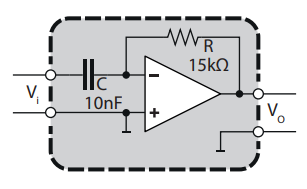
\includegraphics[width=0.5\textwidth]{imagen7.png}
			\caption{Un ejemplo de filtro pasa alto}
		\end{figure}

		\subsubsection{Filtro Pasa Bajo}
		\begin{figure}[H]
			\centering
			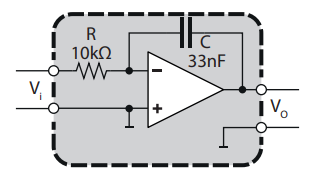
\includegraphics[width=0.5\textwidth]{imagen8.png}
			\caption{Un ejemplo de filtro pasa bajo}
		\end{figure}
	\clearpage	
\end{document}
